\documentclass[11pt,twoside]{report}


%\newif\ifmynotes
%\mynotesfalse
%\mynotestrue

\usepackage{ece586}


%% TOGGLE  Notes
%\newif\ifgnotes
%\anstrue

%\ifmynotes
%	\definecolor{note_text}{rgb}{1,1,1}		
%	\newcommand{\gskip}{\vspace*{1cm}}
%	\newcommand\gnote[1]{\protect\leavevmode\begingroup\Huge\color{note_text}#1\endgroup\ignorespaces}
%	\newenvironment{gnotes}{\Huge\color{red}}{\ignorespacesafterend}
%\else
%	%\newcommand{\gnote}[1]{#1\ignorespaces} 	% make commands do nothing. 
%	\definecolor{note_text}{rgb}{0,0,.7}
%	\newcommand\gnote[1]{\protect\leavevmode\begingroup\color{note_text}#1\endgroup\ignorespaces}
%	\newenvironment{gnotes}{\color{red}}{\ignorespacesafterend}
%%	\newcommand{\gskip}{}
%\fi
%

\newcommand{\bbN}{{\mathbb{N}}}
\newcommand{\bbR}{{\mathbb{R}}}
\newcommand{\bbQ}{{\mathbb{Q}}}
\newcommand{\bbZ}{{\mathbb{Z}}}
\newcommand{\vecnot}{\underline}


\newcommand{\Interior}[1]{\ensuremath{{#1}^{\circ}}}
\newcommand{\Closure}[1]{\ensuremath{\overline{#1}}}
\newcommand{\Complement}[1]{\ensuremath{{#1}^{c}}}

\begin{document}

\lectureheader{2}{Metric Spaces and Topology}



\section*{Overview} 

\begin{itemize}
%\item In this lecture, we consider noisy linear observation model
% \[
% \by = A \bx^\star + \be
% \]
% where:
%\begin{itemize}
%\item $\bx^\star$ is an unknown $n$-dimensional vector belonging to a set $\cX \subseteq \reals^n$. 
%\item $A$ is an $m \times n$ measurement matrix
%\item $\be$ is and $m$-dimensional vector of measurement errors
%\end{itemize}


\item This lecture is based on material in  \cite[Chapter~2]{chamberland:2023EF}.
% and \cite[Parts~I--II]{bloch:2011}


\end{itemize}

\section{Introduction} 

%\section{Logic Systems} 

\begin{itemize}
\item \textbf{Topology:} is the branch of math that quantifies the notation of distance. 
\begin{itemize}
\item Historically, many notions were first considered for the real line, and then subsequently generalized to more abstract spaces, called ``topological spaces''
\item For the purposes of this class, we focus on topologies defined by a metric. 
\end{itemize}

\item \textbf{Definition:} A \textbf{metric} $d$ on a set $X$ is function $d \colon X \times X \to \bbR$ such that
\begin{enumerate}
  \item  $d(x,y) \geq 0 \quad \forall x, y \in X$; with equality iff $x = y$ \hfill (non-negativity)
  \item $d(x,y) = d(y,x) \quad \forall x, y \in X$ \hfill (symmetry)
  \item $d(x,z) \le d(x,y) + d(y,z)  \quad \forall x, y, z \in X$ \hfill (triangle inequality)
\end{enumerate}

\vspace{.2in}
\begin{center}
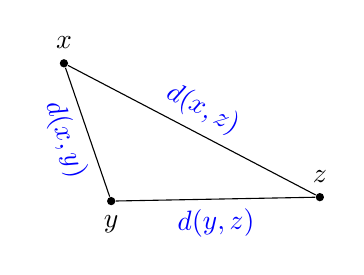
\begin{tikzpicture}%[overlay,remember picture,shift={(12.5,1.5)}]
%\draw[fill=blue!10] (-1,-1) rectangle (3.2,2.2); 
%\draw[fill=blue!10] (-1,-1) rectangle (3.2,2.2); 
%    \node at (2.7,1.6) {$X$};
    \node[circle,label={$x$},fill=black,minimum size=3pt, inner sep=0pt] (a) at (-0.55,1.3) {};
    \node[circle,label={$z$},fill=black,minimum size=3pt, inner sep=0pt] (c) at (2.7,-0.4) {};
    \draw (a) -- (c) node[blue,midway,above,sloped] {$d(x,z)$};


    \node[circle,label=below:{$y$},fill=black,minimum size=3pt, inner sep=0pt] (b) at (0.05,-0.45) {};
    \draw (a) -- (b) node[blue,midway,below,sloped] {$d(x,y)$};
    \draw (b) -- (c) node[blue,midway,below,sloped] {$d(y,z)$};

\end{tikzpicture}\\
Illustration of triangle inequality 
\end{center} 

\item \textbf{Definition:} A \textbf{metric space} $(X,d)$ is a set $X$ along with a metric $d(x,y)$. 

\begin{itemize}
\item The elements of $X$ are called \textbf{points} 
\item $d(x,y)$ is called the \textbf{distance} %between the \textbf{points} $x$ and $y$. 

\end{itemize}
\item \textbf{Examples:}

\begin{itemize}
\item  $X = \bbR$ with \textbf{absolute distance} $d(x,y)  = |x-y|$

\item   $X = \bbR^n$ with \textbf{Euclidean metric}  
\[
d(\vecnot{x},\vecnot{y})=\sqrt{(x_1-y_1)^2 + \ldots + (x_n-y_n)^2}
\]

\item $X$ is condtinuous functions $f \colon [a,b] \to \bbR$ with metric
\[
d(f,g) = \max_{x \in [a,b] } |f(x) -g(x)|
\]
To see this metric satisfies triangle inequality, observe that for $f, g, h$, 
  \begin{align*}
    \max_{x\in [a,b]} | f(x) - h(x) |
    &= \max_{x\in [a,b]} | f(x) - g(x) + g(x) - h(x) |  \\
    &\leq \max_{x\in [a,b]} \left[ |f(x) - g(x)| + |g(x) - h(x)| \right] \\
    &\leq \max_{x\in [a,b]} |f(x) - g(x)| + \max_{x\in [a,b]} |g(x) - h(x)| = d(f,g) + d(g,h)
  \end{align*}

\end{itemize}



\item \textbf{Definition:}  The \textbf{open ball} of radius $\eps > 0$ centered at point $x \in X$ is 
\[
B_d(x,\eps) \coloneqq \{ y \in X \mid d(x,y)  < \eps\} 
\]

\item \textbf{Claim:} For all $a \in B_d(x,\eps)$ there exists $\delta > 0$ such that 
\[
B_d(a,\delta) \subseteq B_d(x,\eps) 
\]
 \item \textbf{Proof:}
 \begin{itemize}
 
 \item Set $\delta = \eps -  d(a,x) > 0$. 
 
 \item For every point $y \in B_d(a, \delta )$ we use the triangle inequality to write 
 \[
 d(x,y) \le d(x,a)  + d(a, y) <d(a,x) + \delta  = \eps 
% d(a,y) <\delta %= \eps -  d(a,x) 
 \]
 \item Hence  $B_d(a,\delta) \subseteq B_d(x,\eps)$
 \end{itemize} 

\end{itemize}
\section{Convergence} 
\begin{itemize}
\item  A \textbf{sequence} of elements from a set $X$  is an infinite list $x_1, x_2, x_3, \dots$ where $x_i \in X$ for $i \in \bbN$ 
\begin{itemize}

\item Can be viewed as a function from domain $\bbN$ to  $X$ 

\item Sometimes denoted $(x_n )_{ n \in \bbN}$% or just $\{x_i\}$ 

\item Sometimes denoted with curly brackets as $\{x_n\}$
\end{itemize}


\item \textbf{Definition:}  A sequence $(x_n)$  in metric space  $(X,d)$  \textbf{converges} to a point $x \in X$% (denoted $x_n \to x$) if,
\[
( \forall \eps > 0) (\exists N \in \bbN) (\forall n \ge N) \quad   d(x,x_n) \le \eps
\]
This is denoted variously as 
\[
\lim_{n\to \infty} x_n = x , \qquad \text{or} \qquad x_n \to x  \text{  as $n \to \infty$}% \qquad \text{or} \qquad x_n \xrightarrow{n\to\infty} x
\]

\item \textbf{Definition:} 
A sequence $(x_n)$ in metric space  $(X,d)$ is \textbf{Cauchy} if
%, for any $\epsilon >0$, there is a natural number $N$ (which may depend on $\epsilon$) such that, for all $m,n > N$,\vspace{-2mm}
%\begin{equation*}
%d \left( x_m, x_n \right) < \epsilon
%\end{equation*}
%Equivalently, 
\[
( \forall \eps > 0) (\exists N \in \bbN) (\forall n,m \ge N) \quad   d(x_n,x_m) \le \eps
\]


\item \textbf{Theorem:} If a sequence  $(x_n)$ in metric space $(X, d)$  is convergent then it is Cauchy 

\item \textbf{Proof:} 
\begin{itemize}
\item Fix any $\eps > 0$. 
\item Since $(x_n)$ converges, there exists $N$ (possibly depending on $\eps$) such that 
\[
d(x,x_n) \le \eps/2 \quad \forall n  \ge N
\]
\item By the triangle inequality, it follows that for all $n,m \ge N$, 
\[
d(x_m, x_n ) \le d(x_m, x) + d(x, x_n) \le  \eps/2 + \eps/2  = \eps 
\]
\item Hence $(x_n)$ is Cauchy. 
\end{itemize}



\end{itemize}


\subsection{Completeness} 

\begin{itemize}

\item \textbf{Question:} Is every Cauchy sequence a convergent sequence?

%\begin{itemize}
%\item YES --- is space is \textbf{complete} 
%\item NO --- otherwise. 
%\end{itemize}

\item \textbf{Example:}  A Cauchy sequence that does not converge 
\begin{itemize}
\item Let $(X, d)$ be rationals $X = \bbQ$ with absolute distance $d(x,y) = |x- y|$. 
\item Construct sequence $x_1, x_2, x_3, \cdots \in \bbQ$ according to 
\[
x_1 = 2, \qquad x_{n+1} = \frac{1}{2} x_n + \frac{1}{x_n} 
\]
\item Can show that $(x_n)$ is a Cauchy sequence and $| c_n - \sqrt{2} | \to 0$. But $\sqrt{2}$ is irrational and to the sequence does not convergence to a limit in $X$. 
\end{itemize}




\item \textbf{Definition:} A metric space $(X,d)$ is  \textbf{complete} if every Cauchy sequence in $(X,d)$ converges to a limit $x \in X$.

\item \textbf{Example:}  The metric space of rationals with absolute distance \emph{is not} complete. 

%\item \textbf{Example:} Consider the sequence $x_n \in \mathbb{Q}$ defined by 
%\[x_1 = 2, \qquad x_{n+1} = \frac{1}{2}x_n +\frac{1}{x_n}
%\]
%For this sequence,  $x_n \to \sqrt{2}$.  Since $\sqrt{2}$ is not rational, this shows the standard metric space of rationals is  \emph{not complete}.
%

\item \textbf{Fact:} The  standard metric space of real numbers with absolute distance  \emph{is} complete



\item \textbf{Theorem:} If $(X,d)$ is a complete metric space and $A \subset X$ is closed  then $(A, d)$ is a complete metric space. 
%A closed subset $A$ of complete metric space $X$ is itself a complete metric space. 

\item \textbf{Proof:}
\begin{itemize}

\item By completeness of $(X,d)$, any Cauchy sequence  $x_n \in A$ converges to a point $x \in X$. 
\item Since $A$ is closed, it contains its limit points and so $x \in A$. 
\item Thus, every Cauchy sequence in $A$ converges to a limit point in $A$. 
\end{itemize}



\color{gray}
\item \textbf{Definition:} 
The \textbf{completion} of a metric space $(X,d_X)$ consists of a complete metric space $(Y,d_Y)$ and an isometry $\phi  \colon X \rightarrow Y$ such that $\phi(X)$ is a dense subset of $Y$.
Moreover, the completion is unique up to isometry.


\item \textbf{Fact:} 
One can always complete a metric space $(X,d)$ by considering Cauchy sequences of elements in $X$.

\color{black}


\item \textbf{Example:}
Let $X=C[-1,1]$ be the space of continuous functions that map $[-1,1]$ to $\mathbb{R}$ and satisfy $\left\| f \right\|_2 < \infty$, where $\left\| f \right\|_2$ denotes the $L^2$ norm \vspace{-3mm}
\begin{equation*}
\left\| f \right\|_2 \coloneqq \left( \int_{-1}^1 |f(t)|^2 dt \right)^{1/2} \vspace{-2mm}
\end{equation*}
\begin{itemize}
\item This set forms a metric space $(X,d)$ when equipped with the distance \vspace{-3mm}
\[ d(f, g)\coloneqq \left\| f - g \right\|_2
= \left( \int_{-1}^1 |f(t) - g(t)|^2 dt \right)^{1/2}  \]
\item  Now, consider the sequence of functions $f_n(t)$ given by
\begin{equation*}
f_n(t) \coloneqq \begin{dcases} 
0,  & t \in \left[ -1, -\tfrac{1}{n} \right] \\
\frac{nt}{2} + \frac{1}{2} & t \in \left( -\tfrac{1}{n}, \tfrac{1}{n} \right) \\
1 & t \in \left[ \tfrac{1}{n}, 1 \right] 
\end{dcases}
\end{equation*}


\item One can show that this is a Cauchy sequence in $(X,d)$ 
\item But, \emph{it does not converge} to a continuous function in $C[-1,1]$
\end{itemize}

\begin{center}
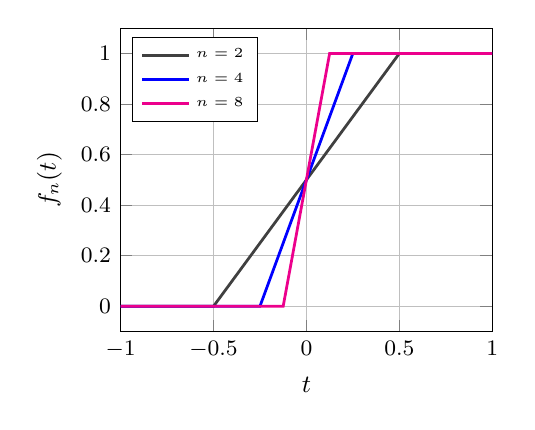
\begin{tikzpicture}%[overlay,remember picture,shift={(10.75,1.5)}]
%\draw[fill=brown!30,rounded corners] (-1.3,-0.9) rectangle (4.1,3.15);
\begin{axis}[
    %title={Continuous Functions},
%    axis background/.style={fill=white},
	small,
	font=\small,
    width=63mm,
    xlabel={$t$},
    xlabel near ticks,
    xmin=-1, xmax=1,
    xmajorgrids,
    ylabel={$f_n(t)$},
    ylabel near ticks,
    ymajorgrids,
    legend style={font=\tiny},
    legend pos=north west]

\addplot[darkgray,line width=1pt] coordinates {
    (-1,0) (-0.5,0) (0.5,1) (1,1)};
\addlegendentry{$n = 2$}

\addplot[blue,line width=1pt] coordinates {
    (-1,0) (-0.25,0) (0.25,1) (1,1)};
\addlegendentry{$n = 4$}

\addplot[magenta,line width=1pt] coordinates {
    (-1,0) (-0.125,0) (0.125,1) (1,1)};
\addlegendentry{$n = 8$}
\end{axis}
\end{tikzpicture}
\end{center}


\end{itemize}




\subsection{Real numbers \& MCT}

\begin{itemize}

\item The statement $x_n \to \infty$ is equivalent to  
\[
\forall M > 0, \, \exists N \in \bbN, \, \forall n \ge N, \, x_n  >  M 
\]

\item The \textbf{extended real numbers} are defined by
\[
\overline{\bbR} = \bbR \cup \{ -  \infty,  \infty\}
\]
\begin{itemize}
\item The set $\overline{\bbR}$ forms a metric  space with metric
\begin{align*}
d_{\overline{\bbR}}(x,y) \coloneqq \left | \frac{ x }{ 1 + |x|}  - \frac{ y}{ 1 + |y|} \right|
% \begin{dcases} 
%- 1, & x = - \infty\\
%\left | \frac{ x }{ 1 + |x|}  - \frac{ y}{ 1 + |y|} \right| , & x \in \bbR
%\end{dcases} 
\end{align*}
where $\frac{x}{1+ |x|}$ evaluates to $-1$ for $x =  - \infty$ and $+1 $ for $x  =  \infty$


\item In the metric space $(\overline{\bbR}, d_{\overline{\bbR}})$ the statement $x_n \to \infty$ correspond to the usual definition of convergence in a metric space, i.e., for all $\eps > 0$ there exists $N \in \bbN$ such that for all $n \ge 
N$,  $d_{\overline{\bbR}}(x_n, \infty) \le \eps$. 

\end{itemize}


\item %\textbf{Definition:} %$For a set $X \subset \bbR$ 
An extended real number $M \in \overline{\bbR}$  is an \textbf{upper bound} for a set $X \subseteq \bbR$ if 
%An upper bound of a set $X \subset \bbR$ is any extended real number $M \in \overline{\bbR}$ such that
\[
x \le M, \quad \forall x \in X
\]



\item The \textbf{supremum} (or least upper bound) of $X\subseteq \bbR$ is the 
%denoted \textbf{$\sup X$} and equals the
 smallest extended real number $M \in \overline{\bbR}$ that $M$ is an upper bound for $X$, i.e., 
 \begin{align*}
 \sup X =  M \quad &  \iff 
 \quad \text{``$M$ is an upper bound'' }  \wedge  \text{ ``$M \le M'$ for every  upper bound $M'$''}\\
 & \iff  \quad    (\forall x \in X, \, x \le M) \,   \wedge \,  (\forall \eps > 0, \,  \exists x \in X,  \,  x > M - \eps)  
 \end{align*}
 
 
 \item The \textbf{infimum} (or greatest lower bound)  is of $X\subseteq \bbR$ is the  largest extended real number $M \in \overline{\bbR}$ that $M$ is an lower bound for $X$, i.e., 
\[
\inf X = - \left(\sup \, -\!X\right), \quad \text{where $-\!X = \{x\in \mathbb{R}\,|-\!x\in X\}$}
\]
 

%\item \textbf{Lemma:} 
%Let $X$ be a metric space and $f \colon X\rightarrow \bbR$ be a function mapping $X$ to the real numbers.
%Let $M = \sup f(A)$ for some non-empty $A \subseteq X$.
%Then, there exists a sequence $x_1,x_2,\ldots \in A$ such that $\lim_n f(x_n) = M$.

\item %\textbf{Definition:}
 The \textbf{maximum} of $X\subseteq \bbR$ is the largest value contained in the set.
It equals the supremum if $\sup X \in X$ and it is \emph{undefined} otherwise.
\[
\max X = M \quad \iff \quad  (\sup X =  M) \wedge (M \in X)
\]


\item %\textbf{Definition:}
 The \textbf{minimum} of $X\subseteq \bbR$ is the smallest value contained in the set.
It equals the infimum if $\inf X \in X$ and it is \emph{undefined} otherwise.
\[
\min X = M \quad \iff \quad  (\inf X =  M) \wedge (M \in X)
\]



\item \textbf{Examples:} 
\begin{itemize}
\item If $X = [1,2) \subset \mathbb{R}$ then
\begin{align*}
\sup X = 2, \qquad \max X = \text{undefined}, \qquad \inf X = 1, \qquad \min X = 1
\end{align*}
%
%\]has $\sup X = 2$ and $\max X$ undefined. 
\item If $f(x)=\frac{1}{2-x}$ then $f(X) = [1, \infty)$ and so 
\[
\sup f(X) = \infty, \qquad \max f(X) = \text{undefined}, \qquad \inf f(X) = 1, \qquad \min f(X) = 1
\]
%$f(X) = [1,\infty)$ and $\sup f(X) = \infty$.
\end{itemize}

\item \textbf{Remark:} The supremum and infimum always well-defined but may equal $\pm \infty$

%\begin{itemize}
%\item \textbf{infimum} (or greatest lower bound)  is 
%\[
%\inf X = - \left(\sup \, -\!X\right), \quad \text{where $-\!X = \{x\in \mathbb{R}\,|-\!x\in X\}$}
%\]
%\item \textbf{minimum} is the smallest element contained in the set
%\[
%\min X = - \left(\max \, -\!X \right) \quad \text{ if it exists}
%\]
%\item supremum and infimum always well-defined but may equal $\pm \infty$
%\end{itemize}

\item \textbf{Monotone Convergence Theorem (MCT):} If $(x_n)_{n \in \bbN} $ is a nondecreasing sequence of real numbers that is bounded from above, i.e., $x_1 \le x_2 \le x_3 \le \cdots \le x_n \le M$ for all $n$, then it converges to its supremum. 
 

\item \textbf{Proof} 
\begin{itemize}
\item Assume w.l.o.g.\ that $M = \sup \{x_n \mid n \in \bbN \}$ is the least upper bound.

\item From the definition of the supremum, $x_n \le M$ and for all $\eps > 0$ there exists $N \in \bbN$ such that $x_N > M -\eps$. 

\item Since $\{x_n\}$ is non-decreasing, this implies that $x_n \ge M -\eps$ for all $n \ge N$. 

\item Thus, $|x_n - M| \le \eps$ for all $n \ge N$ and so $x_n \to M$. 


\end{itemize}

\end{itemize}




\section{Metric topology} 

\begin{itemize}

\item \textbf{Definition:}  Let $W$ be a subset of a metric space $(X,d)$.
The set $W$ is called \textbf{open} if%, for every $w_0 \in W$, there is an $\epsilon>0$ such that 
\[
(\forall w  \in W) ( \exists  \eps > 0) \quad B_d (w,\epsilon) \subseteq W
\]





\item \textbf{Definition:} A subset $W$ of metric space $(X,d)$ is \textbf{closed} if its complement $W^c = X-W$ is open.



\begin{center}
%\scalebox{0.7}{%
\begin{tikzpicture}[scale=0.8]
\draw[very thick] (-0.5,-1.5) rectangle (3.5,2) node[below left=0.2cm and 0.2cm] {$X$};
\draw [thick,dashed,fill=blue!10] plot [smooth cycle] coordinates {(0,0) (1,1) (3,1) (2,0) (2,-1)} node[above left=0.65cm and 0.15cm] {open};
\end{tikzpicture}
\hspace{5mm}
%\scalebox{0.7}{%
\begin{tikzpicture}[scale=0.8]
\draw[very thick] (-0.5,-1.5) rectangle (3.5,2) node[below left=0.2cm and 0.2cm] {$X$};
\draw [thick,fill=blue!10] plot [smooth cycle] coordinates {(0.5,0) (1,1.5) (2.5,1) (2.5,0) (1.5,-1)} node[above left=0.75cm and -0.6cm] {closed};
\end{tikzpicture}
\hspace{5mm}
%\scalebox{0.7}{%
\begin{tikzpicture}[scale=0.8]
\draw[very thick] (-0.5,-1.5) rectangle (3.5,2) node[below left=0.2cm and 0.2cm] {$X$};
%\clip (1,1) circle(0.5);
\fill[blue!10,even odd rule] plot [smooth cycle] coordinates {(0.5,0) (1,1.5) (2.5,1) (2.5,0) (1.5,-1)} (1.5,0.5) circle (0.5);
\draw[thick,dashed] (1.5,0.5) circle (0.5);
\draw [thick] plot [smooth cycle] coordinates {(0.5,0) (1,1.5) (2.5,1) (2.5,0) (1.5,-1)} node[above left=0.35cm and -0.6cm] {neither};
\end{tikzpicture}
\end{center}  



\item \textbf{Theorem:}  For any metric space $(X,d)$,
\begin{enumerate}
\item $\emptyset$ and $X$ are open sets
\item any union of open sets is open
\item any finite intersection of open sets is open
\end{enumerate}

\item \text{Proof:}

\begin{itemize}

\item  $\emptyset$ is open because the ``for all'' qualifier over the empty set is always true: 
\[
\forall w_0 \in \emptyset\,  \big( \underbrace{ \exists  \eps > 0, \,  B_d (w_0,\epsilon) \subseteq W }_\text{this part doesn't matter}  \big) 
\] 

\item $X$ is open because $B_d(w_0, \eps) \subseteq X$ is always true definition

\item To show finite union it is sufficient to consider the union of two open sets
\[
W = W_1 \cup W_2
\]
For all $w_0 \in W$, either $w_0 \in W_1$ or $w_0 \in W_2$.  Assume w.l.o.g.\ that $w_0 \in W_1$. Then 
\[
\exists \eps > 0, \; B_d(w_0,\eps) \subseteq W_1 \subseteq W
%\text{$W_1$ is open} \quad \implies \quad \forall x \in W_1, \exists 
\]
\end{itemize}


\item \textbf{Example:} An \emph{infinite} intersection of open sets need not be open. For example if 
\[
A_n = (-\tfrac{1}{n} , \tfrac{1}{n})
\]
then
\[
\bigcup_{n} A_n = \{ 0\} 
\]
This is not an open subset of the reals. 


\item \textbf{Example:} Let $(X, d)$ be standard real metric space and $a < b$ real numbers. 
\begin{itemize}
\item The interval $I_1 = (a, b)$ is open, 
\[
\forall x \in (a, b) ,  \quad B_d(x, \min\{ |a-x|, |b-x| \}  ) \subset (a,b) 
\]

\item The interval $I_2 = (a, \infty)$ is open

\item The interval $I_3 = [a, b)$ is not open because 
\[
\forall \eps >0, \qquad B_d(a,\eps)  \text{  contains some point not in $[a,b)$} 
\]

\end{itemize}


\item \textbf{Example:} Let $(X,d)$ be metric space with finite set $X = \{ x_1, x_2, \dots , x_N\}$ and metric
\[
d(x,y) = \begin{dcases} 0, & x  = y\\
1, & x \ne y 
\end{dcases}
\]
%For a subset $A \subseteq X$ we have the following: 
\begin{itemize}
\item For every set $W \subseteq X$, we have 
%We have %For every $x \in A$ there exists $\eps > 0$  (the choice $\eps = 1/2$ suffices) such that 
\[
\forall x \in W, \quad B_d(x,\tfrac{1}{2}) = W \quad \implies \quad \text{$W$ is open} 
\]
\item By the same argument, $X  - W$ is also open, and thus ever subset is also closed. 
%$0 < \eps < 1$ and any $x \in A$ we have $B_d(x,\eps) = A$. Thus $A$ is open. 
\end{itemize}



\item \textbf{Definition:} Let $(X, d)$ be a metric space and $W$ a subset of $X$
\begin{itemize}
\item A point $x\in X$ is a \textbf{limit point} of $W$ if
\[
 \forall \delta > 0, \quad B_d(x, \delta) \cap W \text{ contains some point besides $x$}
%  \text{$\{ w \in W \mid d(x,w) \le \delta \}$ contains some point besides $x$}
\]
Equivalently, there exists a sequence $w_1, w_2, w_3 , \dots$ in $W \setminus \{x\}$ that has distinct elements (i.e., $w_n \ne w_m$ for all $n \ne m$) and converges to $x$. 

\item A point $x\in X$ is an \textbf{isolated point} of $W$ if %$x \in W$ and 
 %A point that is not a limit point is called an \textbf{isolated point}. Equivalently, a point $x\in W$ is an isolated point of $W$ if
\[
\exists \delta > 0, \quad B_d(x, \delta) \cap W = \{ x\}
\]
From this definition, %we see that $x$ is an isolated point only if  $x \in W$ and and so 
we see that every isolated point is an element of $W$. 


\end{itemize}


%\item For the following definitions, let $(X,d)$ be a metric space and $W$ be a subset of $X$


%\item \textbf{Definition:} % For a metric space $(X, d)$ and subset $W \subseteq X$, 
%A point $x\in X$ is a \textbf{limit point} of $W$ if
%\[
% \forall \delta > 0, \quad B_d(x, \delta) \cap W \text{ contains some point besides $x$}
%%  \text{$\{ w \in W \mid d(x,w) \le \delta \}$ contains some point besides $x$}
%\]
%Equivalently, $\exists$ a sequence $w_1, w_2, \dots \in W \setminus \{x\}$ of \emph{distinct} elements that converges to $x$. 
%
%\item \textbf{Definition:} A point $x\in X$ is an \textbf{isolated point} of $W$ if %$x \in W$ and 
% %A point that is not a limit point is called an \textbf{isolated point}. Equivalently, a point $x\in W$ is an isolated point of $W$ if
%\[
%\exists \delta > 0, \quad B_d(x, \delta) \cap W = \{ x\}
%\]
%From this definition, %we see that $x$ is an isolated point only if  $x \in W$ and and so 
%we see that every isolated point is an element of $W$. 

\item \textbf{Theorem:} For a metric space $(X, d)$ the following are equivalent: 
\begin{enumerate}[(i)]
\item $W$ is closed %(i.e., $X - W$ is open)
\item $W$ contains all of its limit points. 
\end{enumerate}

%, a subset $W \subseteq X$ is closed if and only if it contains all of its limit points. 

\item \textbf{Proof of (i) $\implies$ (ii)}
\begin{itemize}
\item Fix any $x \in X - W$. 
\item If $W$ is closed then  $X - W$ is open, and  $\exists \eps > 0$ such that $B_d(x,\eps) \subseteq X - W$. 
\item Accordingly,   $d(x,w) > \eps$ for all $w \in W$, and so $x$  cannot be a limit point of $W$. 
%\item We have shown that every $x \in X - W$ is not a limit point of $W$. This 
%\[
%\neg \left( \exists x \in X - W,  \quad \text{$x$ is limit point of $W$} \right)  \quad \iff \quad \neg \left( \exists x \in X - W,  \quad \text{$x$ is limit point of $W$} \right)
%\]
%\item If $x \in X$ is a limit point of $W$ were not closed, then there would exist some point $w \in X- 
\end{itemize}


%A point $x_0 \in X$ is a \textbf{limit point} of $W$ if there is: \\  ~~a sequence of distinct elements, $w_1,w_2,\ldots\in W$, that converges to $x_0$.

\item \textbf{Definition:} The  \textbf{interior} of $W$ is the set 
\[
\Interior{W} = \{ w \in W \mid \exists \eps > 0, \, B_d(w, \eps) \subseteq W\} 
\]
%In other words, a point $w_0 \in W$ is in the \textbf{interior} of $W$ if and only if 
%\[
%\text{$\exists \delta >0$ such that $B_d (w_0,\delta) \subseteq W$}
%\]

\item \textbf{Definition:} The  \textbf{closure} of $W$ is the set 
%\[
%\Closure{W} = \{ x\in X \mid \forall \delta > 0, \, \exists w \in W, \,  d(w, y)  < \delta \} 
%\]
\[
\Closure{W} = \{ x\in X \mid \forall \eps > 0, \,  B_d(x,\eps) \cap W \ne \emptyset \} 
\]
i.e., the closure is the union of $W$ and all of its limit points. 

\item \textbf{Definition:} The  \textbf{boundary} of $W$ is the set 
\[
\partial W = \Closure{W} - \Interior{W}
\]


%\item \textbf{Claim:}  The interior is an open set.
%
%\item \textbf{Proof:} 
%\begin{itemize}
%\item Fix any $w \in \Interior{W}$
%\item By definition, there exists $\eps > 0$ such that $B_d(w,\eps) \subseteq W$
%\end{itemize}


\item \textbf{Properties:} 

\begin{itemize}
\item The interior is an open set. 
\item Every point in $W$ is either an interior point or a boundary point. 
\item  For $x \in \partial W$ and  $\delta>0$, the ball $B_d (x,\delta)$ contains a point in $W$ and a point not in $W$

\end{itemize}
%\item  \textbf{Definition:}  %The closure of $W$ is the set 
%A point $x_0\in X$ is in the \textbf{closure} of $W$ (denoted $\Closure{W}$) if
%\[\text{$\forall \delta >0$, there is a $w_0\in W$ such that $d(x_0,w_0)<\delta$}
%\]

\item \textbf{Examples} 
\[
\text{[Illustration of limit points, isolated points, interior, closure, boundary]}
\]

\begin{center}
\begin{tikzpicture}%[overlay,remember picture,shift={(12.5,0.25)}]
%\begin{scope}[scale=0.6]
\draw[very thick] (-0.5,-1.5) rectangle (3.5,2) node[below left=0.1cm and 0.1cm] {\small $X$};
\fill[blue!10,even odd rule] plot [smooth cycle] coordinates {(0.5,0) (1,1.5) (2.5,1) (2.5,0) (1.5,-1)} (1.5,0.5) circle (0.5);
\draw[thick] (1.5,0.5) +(-80:0.5) arc (-80:80:0.5);
%\draw[thick] (1.5,0.5) arc (-20:40:0.5);
%\path[thick,dashed] (1.5,0.5) coordinate (A) (1.5,0.5) coordinate (B) (60:0.5) coordinate (C) (120:0.5) coordinate (D);
\draw[thick,dashed] (1.5,0.5) circle (0.5);
\draw [thick,dashed] plot [smooth cycle] coordinates {(0.5,0) (1,1.5) (2.5,1) (2.5,0) (1.5,-1)} node[above left=0.1cm and -0.3cm] {\small $W$};
%\path[draw,thick] (0.5,0) --  (1,1.5) --  (2.5,1);
%\end{scope}

\end{tikzpicture}

The boundary is the union of the dashed and solid lines.
\end{center}


%\item Properties: 
%\begin{itemize}
%  \item The interior $\Interior{W}$ is open (see definition)
%  \item $W$ is closed if and only if it contains all of its limit points
%  \item Closure $\Closure{W}$ equals union of $W$ and all its limit points (thus is closed)
%\end{itemize}


%  \item  The Boundary
%  \begin{itemize}
%
%    \item For $W \subseteq X$, the \textbf{boundary} $\partial W$ is the closure minus the interior $\Closure{W} - \Interior{W}\!\!\!$
%    \item Thus, the closure is the union of the set and its boundary
%    \item In the figure, the boundary is the union of the dashed and solid lines
%    \item Alternatively, a point $x\in X$ is on the \textbf{boundary} of $W$ if, for all $\delta>0$, $B_d (x,\delta)$ contains a point in $W$ and a point not in $W$
%
%  \end{itemize}


\item \textbf{Definition:} A subset $A$ of a metric space $(X,d)$ is \textbf{dense} in $X$ if every $x\in X$ is a limit point of the set $A$.
This is equivalent to the closure $\overline{A}$ being equal to $X$.
% \gpt{Suggested replacement from the revised book: ``$A$ is dense in $X$ if every nonempty open ball in $X$ intersects $A$, equivalently $\overline A=X$.'' Requiring every point to be a limit point is too strong when isolated points are present.}


\item \textbf{Example:}
The rational numbers are a dense subset of the real numbers because every real number is the limit of a sequence of rational numbers.




\end{itemize}



\section{Continuity} 
\begin{itemize}


\item \textbf{Definition:} Let $f \colon X \to Y$ be a function between metric spaces $(X, d_X)$ and $(Y,d_Y)$

\begin{itemize}

\item  $f$ is \textbf{continuous at point  $x_0 \in X$} if %for any $\epsilon> 0$, there exists a $\delta >0$ such that, for all $x\in X$ satisfying $d_X(x_0,x)< \delta$, we find $d_Y \left( f(x_0),f(x) \right) < \epsilon$
%\[
%\forall \eps > 0, \, \exists \delta > 0\, \forall x \in B_{d_X}(x_0, \delta) , \, d_Y\big( f(x_0) , f(x) \big)  < \eps 
%\]
%\[
%(\forall \eps > 0)  \, (\exists \delta > 0) \, ( \forall x \in B_{d_X}(x_0, \delta) )  \quad  d_Y\big( f(x_0) , f(x) \big)  < \eps 
%\]
\[
\forall \eps > 0,   \, \exists \delta > 0,  \,  \forall x \in X ,  \quad \big( d_X(x_0,x) < \delta \; \implies \;   d_Y\big( f(x_0) , f(x) \big)  < \eps \big)
\]
%In other words, for $\eps > 0$ there exists $\delta > 0$ such that 
%\[
%d_X(x_0, x) < \delta \implies d_Y(f(x_0), f(x)) < \eps
%\]

\item   $f$ is \textbf{continuous} if it is continuous at points in $X$, i.e., 
%\[
%(\forall x_0 \in X)\, (\forall \eps > 0)  \, (\exists \delta > 0) \, ( \forall x \in B_{d_X}(x_0, \delta) )  \quad  d_Y\big( f(x_0) , f(x) \big)  < \eps 
%\]
\[
 \forall \eps > 0,   \, \forall x_0 \in X, \, \exists \delta > 0,  \,  \forall x \in X ,  \quad \big( d_X(x_0,x) < \delta \; \implies \;   d_Y\big( f(x_0) , f(x) \big)  < \eps \big)
\]


\item   $f$ is \textbf{uniformly continuous} if
\[
\forall \eps > 0,  \, \exists \delta > 0,  \, \forall x_0, x  \in X\,  ,  \quad \big( d_X(x_0,x) < \delta \; \implies \;   d_Y\big( f(x_0) , f(x) \big)  < \eps \big)
\]
In other words, $\delta$ can be chosen independently of $x_0$.

\item   $f$ is \textbf{Lipchitz continuous}  on $A \subseteq X$ if there exists a constant $L \in \bbR$ such that
\[
d_Y(f(x), f(x')) \le L d_X(x,x') \quad \text{for all $x,x' \in A$}
\]

\end{itemize}




\item \textbf{Theorem:} The following statements are equivalent: 
\begin{enumerate}[(i)]
\item  $f$ is continuous at $x_0$. 
%, then $f(x_n) \to f(x_0)$ for all sequences $x_1,x_2,\ldots \in X$ such that $x_n \to x_0$.
\item  $f(x_n) \to f(x_0)$ for all sequences $x_1,x_2,\ldots  \in X$ such that $x_n \to x_0$
\end{enumerate}

\item \textbf{Example:} Let $f \colon (0,1] \to [1,\infty)$ be defined by
\[
f(x) = \frac{1}{x} 
\]
\begin{itemize}
\item Is this function well defined?

\item Is this function continuous?\\

YES -- For $x_0 \in X$ and $\eps  >0$ set $\delta = \frac{ \eps x_0^2}{ 1 + \eps x_0}$. Then, for all $x \in B_d(x_0, \delta)$,  
  \[ \left| \frac{1}{x}-\frac{1}{x_0} \right| = \left| \frac{x_0 - x}{x \, x_0} \right| < \frac{\frac{\epsilon x_0^2}{1+\epsilon x_0}}{x_0 \big( x_0 - \frac{\epsilon x_0^2}{1+\epsilon x_0} \big)} = \frac{\epsilon}{(1+\epsilon x_0)( 1 - \frac{\epsilon x_0}{1+\epsilon x_0})} = \epsilon\] 

\item Is this function uniformly continuous? \\

NO -- The negation of uniformly continuous is
 \[
 \exists \epsilon >0, \forall \delta >0, \exists x_0, x  \in X \text{ s.t. }  ( |x-x_0|<\delta )  \wedge   ( |f(x)-f(x_0)|\ge \epsilon)
  \]
Let $\epsilon = 1$. Given any  $\delta > 0$, set $x_0 = \min\big\{ \frac{1}{2},\frac{\delta}{2} \big\}$ and  $x=2 x_0$.  Then 
\[
| x - x_0 | = x_0 \leq \frac{\delta}{2}
\]
and so
\[
 \left| \frac{1}{x}-\frac{1}{x_0} \right| = \left| \frac{x_0 - x}{x \, x_0} \right| = \frac{x_0}{x \, x_0} = \frac{1}{x} = \max\left\{1,\frac{1}{\delta}\right\} \ge 1  = \eps
 \]

\end{itemize}

\begin{center}
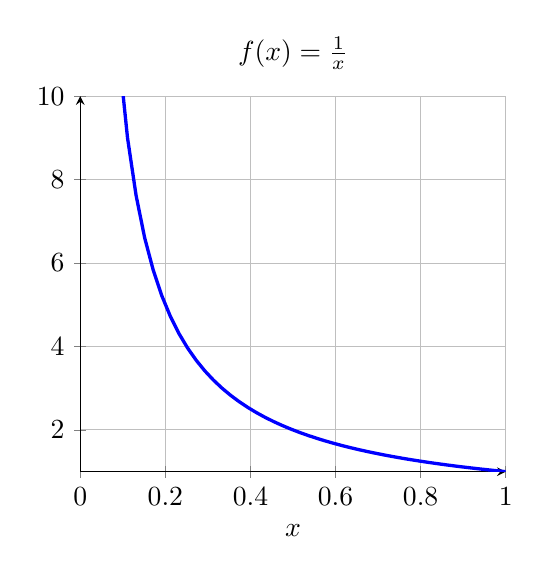
\begin{tikzpicture}%[overlay,remember picture,shift={(11.75,1.0)}]
  \begin{axis}[
    height=2.5in,
    width=2.75in,
    axis lines = left,
    grid=major,
    ymax=10,
    xmin=0,
    xlabel = \(x\),
    title = {$f(x)=\frac{1}{x}$},
    %ylabel = {\(f(x)\)},
  ]
  \addplot [
    very thick,
    domain=0.01:1, 
    samples=50, 
    color=blue,
  ]
  {1/x};
  \end{axis}
\end{tikzpicture}
\end{center}


\item \textbf{Example:} Let $f \colon [0,1] \to [0,1]$ be defined by
\[
f(x) = \sqrt{x} 
\]
\begin{itemize}
\item Is this function well defined?

\item Is this function continuous?
\item Is this uniformly continuous?\\

YES --- Given $\eps > 0$ set $\delta = \eps^2$ then, for all $|x-y|  < \delta$, it follows that
\[
|\sqrt{x} - \sqrt{y} | = \sqrt{ |\sqrt{x} - \sqrt{y} | |\sqrt{x} - \sqrt{y} | }  \le  \sqrt{ |\sqrt{x} - \sqrt{y} | |\sqrt{x} + \sqrt{y} | }  = \sqrt{ | x- y|}  < \eps 
\]
\item Is this function Lipchitz continuous?\\

NO --   Lipchitz means that
\[
\sup \left\{ \frac{ |f(x) - f(y)| }{ |x- y| } \mid x, y \in X,  \,  x \ne y \right \}  < \infty
\]
However, 
\[ \sup_{\substack{x,y\in X \\ x\neq y}} \frac{|\sqrt{y} - \sqrt{x}|}{|y-x|} \geq \sup_{z\in (0,\frac{1}{2}]} \frac{\sqrt{z^2 + z}-\sqrt{z^2}}{(z^2+z)-z^2} \geq \sup_{z\in (0,\frac{1}{2}]}  \frac{1}{\sqrt{z}} - 1  = + \infty
\]

\end{itemize}


\begin{center}

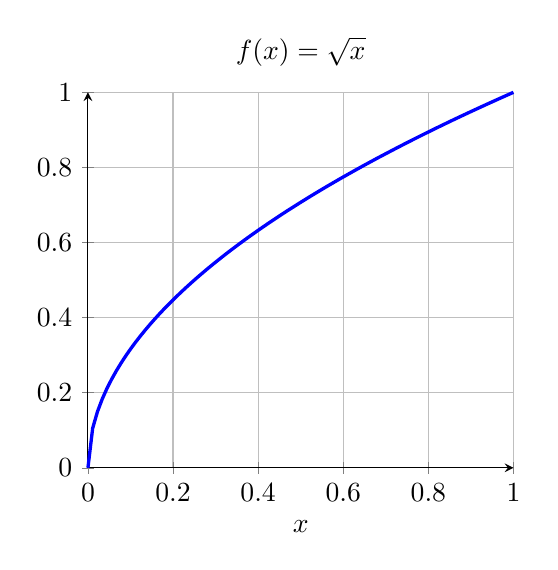
\begin{tikzpicture}%[overlay,remember picture,shift={(11.70,0.85)}]
  \begin{axis}[
    height=2.5in,
    width=2.75in,
    axis lines = left,
    grid=major,
    xlabel = \(x\),
    title = {$f(x)=\sqrt{x}$},
    %ylabel = {\(f(x)\)},
    clip =false,
  ]
  \addplot [
    very thick,
    domain=0:1, 
    samples=91, 
    color=blue,
  ]
  {(x)^(0.5)};
  \end{axis}
\end{tikzpicture}
\end{center}




\item \textbf{Sequence of functions:} Let $(f_n)_{n \in \bbN}$  and $f$ be functions from metric space $(X, d_X)$ to metric space $(Y, d_Y)$. 
\begin{itemize}
\item \textbf{pointwise convergence} 
\[
\forall x \in X, \quad \lim_{n \to \infty} f_n(x) = f(x) 
\]

\item \textbf{uniform convergence} 
\[
(\forall \eps > 0 )(\exists N \in \bbN)  (\forall n \ge N) ( \forall x \in X) \quad d_Y(f_n(x), f(x)) \le \eps 
%\forall x \in X, \quad \lim_{n \to \infty} f_n(x) = f(x) 
\]

\end{itemize}



\item \textbf{Theorem:} If each $f_n$ is continuous and the sequence $\{f_n\}$ converges uniformly to $f \colon X \to Y$ then the limit function $f$ is continuous. 



\item \textbf{Counter example:} Consider sequence $f_n \colon [0,1] \to \bbR$ defined by 
\[
f_n(x) = x^n 
\] 
\begin{itemize}
\item Is each $f_n$ continuous? \\

YES --  can use proof by induction. Show that $f_1$ is continuous. And that if $f_n$ is continuous then $f_{n+1}(x)  = x \cdot f_n(x)$ is also continuous. 

\item Does $f_n$ converge to a limit $f$? \\

YES -- For all $x \in [0,1)$ we have $f_n(x) \to 0$ and also $f_n(0) = 1$ for all $n$. 

\item Does $f_n$ converge to limit $f$ is that is also continuous?\\\

NO! Here, we see that the sequence $f_n$ is continuous but \emph{not} uniformly continuous. 
\end{itemize}



\end{itemize}





\subsection{Contraction} 



\begin{itemize}

\item \textbf{Definition:} Let $A$ be a subset of a metric space $(X,d)$ and $f \colon X \rightarrow X$ be a function. Then, $f$ is a \textbf{contraction} on $A$ if $f(A) \subseteq A$ and there exists a constant $\gamma < 1$ such that
\[
d \left( f(x),f(y) \right) \le \gamma  d(x,y), \quad \text{for all $x,y \in A$} 
\]



\item \textbf{Example:} If $X=[0,1]$  and $f(x) = 1 - x/2$ then 
%with absolute distance.
%Define $f\colon X \to X$
%\[
%f(x) = 1-\frac{1}{2}x
%\]
%and observe that
 \[
 f(X) = [\tfrac{1}{2},1] \subset X \qquad \text{and} \qquad 
  d\big(f(x),f(y)\big)=|f(x)-f(y)| = \frac{1}{2}|x-y|
 \] 


\begin{center}
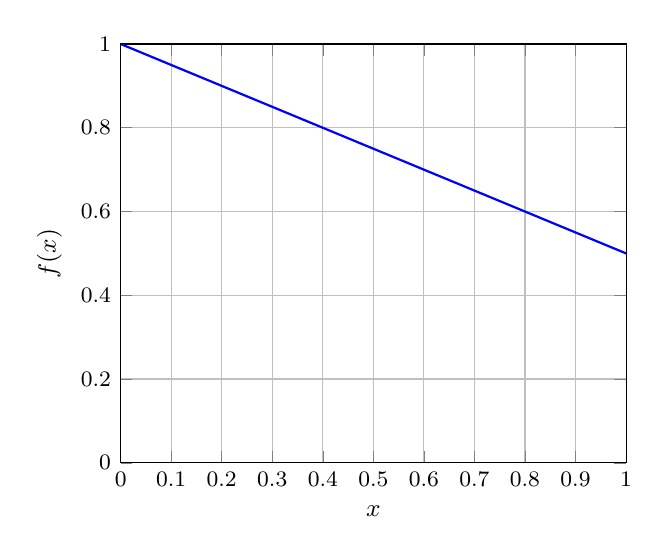
\begin{tikzpicture}%[overlay,remember picture,shift={(12.5,-0.5)}]
\begin{axis}[
	small,
	font=\small,
    width=80mm,
    xlabel={$x$},
    xlabel near ticks,
    xmin=0, xmax=1,
    xmajorgrids,
    ylabel={$f(x)$},
    ylabel near ticks,
    ymin=0,
    ymax=1,
    ymajorgrids,
    legend style={font=\tiny},
    legend pos=north west]

    \addplot[blue,thick] { 1 - x/2 };
\end{axis}
\end{tikzpicture}
\end{center}

\item \textbf{Contraction Mapping Theorem}
Let $(X,d)$ be a complete metric space and $f$ be a contraction on a closed subset $A \subseteq X$.
% \gpt{Suggested cut/paste theorem hypothesis: ``Let $(X,d)$ be complete, let $A\subseteq X$ be nonempty and closed, and let $f\colon X\to X$ satisfy $f(A)\subseteq A$ and $d(f(x),f(y))\leq\gamma d(x,y)$ for all $x,y\in A$, with $0\leq\gamma<1$.''}
Then, 
\begin{itemize}
\setlength\itemsep{3mm}
  \item $f$ has a unique fixed point $x^* \in A$ such that $f(x^*) = x^*$ and the sequence $x_{n+1} = f(x_n)$ converges to $x^*$ from any initial $x_1 \in A$
  \item Also, $x_n$ satisfies the error bounds (for contraction coefficient $\gamma$): \vspace{-2mm} \begin{align*} d(x^*,x_n) &\le \gamma^{n-1} d(x^*,x_1) \\ d(x^*,x_{n+1}) &\leq  \frac{ \gamma}{ 1- \gamma} d(x_n,x_{n+1})
   \end{align*}
\end{itemize}


\item \textbf{Proof of uniqueness}

\begin{itemize}
\item Suppose that $x, y \in A$ are two fixed points in $A$, i.e., $f(x) = x$ and $f(y) = y$. Then, 
\[
d(x,y) = d(f(x),f(y)) \le \gamma d(x,y) 
\]
\item Since $0 <  \gamma <1$ this is possible only if $d(x,y) = 0$ and so $x$ and $y$ are the same fixed point. 
\end{itemize}

\item \textbf{Proof of existence}

\begin{itemize}
\item  By induction, we have 
\[
d(x_{n}, x_{n+1}) = d(f(x_{n-1}), f(x_n)) \le \gamma d(x_{n}, x_{n+1}) 
\]
% \gpt{Suggested cut/paste correction: the last factor must be $d(x_{n-1},x_n)$, so the line reads $d(x_n,x_{n+1})\leq\gamma d(x_{n-1},x_n)$.}
and so 
\[
d(x_{n}, x_{n+1}) \le \gamma^{n-1} d( x_1,x_2)
\]
\item  For all $m , n \in \bbN$ with $m <  n$ we have, 
\begin{align*}
d(x_m, x_n) &\le d(x_m, x_{m+1}) + d(x_{m+1},  x_n) \\
& \le \sum_{i=m}^{n-1} d(x_i, x_{i+1})  \\
& \le \sum_{i=m}^{n-1} \gamma^{i-1}  d(x_1, x_2)  \\
& \le \frac{ \gamma^{m-1}}{ 1- \gamma} 
\end{align*}
Thus, the sequence $(x_n)$ is Cauchy. 

\item By the assumption that $(X, d)$ is complete, ever Cauchy sequence converges to some limit $x^* \in X$. 

\item Since $f$ is continuous, it follows that 
\[
f(x_n) \to f(x^*)
\]
\item Thus, the limit $x^*$ is the unique fixed point
\[
 0 = \lim_{n \to \infty}   ( x_{n+1}  - x_{n}  )  =  \lim_{n \to \infty}   ( f(x_{n})  - x_{n}  ) =  f(x^*) - x^*% \left( \lim_{n \to \infty}    f(x_n) \right)  -\left( \lim_{n \to \infty}  x_{n}  \right) 
\]
\end{itemize}



\item \textbf{Example:}  Let $X = \bbR$, $A  = [0,1]$,   and $f \colon X \to X$ be 
\[
f(x)  = \cos(x)
\]
\begin{itemize}

\item  Verify that  
\[
\cos(A) = [\cos(1), 1] \subseteq A
\]


\item By mean value theorem, 
\[
f(y) - f(x)  = (y-x) f'(t), \qquad f'(t) = \sin(t) , \qquad \max_{t \in A} |\sin(t)| = \sin(1) \le 0.85
\]
\item Thus, 
\[
| \cos(x) - \cos(y) | \le 0.85 |y - x| , \quad \text{for all $x,y \in [0,1]$}
\]
and so $f(x)$ is a contraction on $A$

\end{itemize}
\begin{center}
\input{figures/cos_contract}
\end{center}
%  
\includegraphics[width=\textwidth]{figures/ch2_contraction_mapping}
  
\end{itemize}


\section{Compactness} 

\begin{itemize}




\item The following statements are true for a metric space $(X,d)$ if $X$ is a finite set, but false if $X$ is an infinite set: 
\begin{enumerate}[(i)]
\item All functions are bounded: For every function $f \colon X \to \bbR$, 
\[
%\forall f \colon X \to \bbR, \, 
\exists M \in \bbR, \, \forall x \in X, \quad f(x) \le M
\]
\item All functions attain a maximum: For every function $f \colon X \to \bbR$, 
\[
%\forall f \colon X \to \bbR, \, 
\exists x_0 \in X, \, \forall x \in X, \quad f(x_0) \ge f(x) 
\]
\item All sequences have constant subsequences: For every sequence $x_1, x_2, x_3, \ldots \in X$ there is a subsequence $x_{n_1}, x_{n_2}, x_{n_3}$ that is constant, 
\[
x_{n_1} = x_{n_2} = \dots = x\quad \text{for some $x \in X$}
\]

\item All covers have finite subcovers: For any cover of $X$, i.e., a (possibly infinite) collection of subsets  $V_1, V_2 , V_3 , \ldots \subset X$ such that  $\cup_n V_n  = X$, then there  a exist  \emph{finite} sub-collection $V_{n_1}, V_{n_2}, \dots, V_{n_N}$ that still cover $X$, i.e., 
\[
X = \bigcup_{n = 1}^N V_n 
\]
\end{enumerate}

\item \textbf{Question:} Are there certain types of \emph{infinite} sets for which some modified version of the above statements still hold?  How should these be defined?


\item \textbf{Answer:}  The concept of a \textbf{compactness} allows such a generalization. The following statements are true if $(X,d)$ is a \emph{compact} metric space, but false if it is not compact.  
\begin{enumerate}[(i)]
\item All \emph{continuous} functions are bounded: 
%For every function $f \colon X \to \bbR$, 
%\[
%%\forall f \colon X \to \bbR, \, 
%\exists M \in \bbR, \, \forall x \in X, \quad f(x) \le M
%\]
\item All \emph{continuous} functions attain a maximum: 
%For every function $f \colon X \to \bbR$, 
%\[
%%\forall f \colon X \to \bbR, \, 
%\exists x_0 \in X, \, \forall x \in X, \quad f(x_0) \ge f(x) 
%\]
\item All sequences have \emph{convergent}  subsequences: 
 For every sequence $x_1, x_2, x_3, \ldots \in X$ there is a subsequence $x_{n_1}, x_{n_2}, x_{n_3}, \ldots$ such that  
\[
x_n \to x \quad \text{for some $x \in X$}
\]
[This is called the Bolzano-Weierstrass Theorem] 

\item All \emph{open} covers have finite subcovers: [This is the general definition of compactness!]
%For any cover of $X$, i.e., a (possibly infinite) collection of subsets  $V_1, V_2 , V_3 , \dots \subset X$ such that  $\cup_n V_n  = X$, then there  a exist  \emph{finite} sub-collection $V_{n_1}, V_{n_2}, \dots, V_{n_N}$ that still cover $X$, i.e., 
%\[
%X = \bigcup_{n = 1}^N V_n 
%\]
\end{enumerate}



\item \textbf{Definition:} A metric space $(X,d)$ is \textbf{totally bounded} if, for any $\epsilon > 0$, there exists a finite set of radius-$\epsilon$ balls that cover $X$, i.e., 
\[
\forall \eps > 0, \exists N \in \bbN,   x_1, x_2, \dots , x_N \in X, \qquad 
\bigcup_{x\in S} B_d (x,\epsilon) = X
\]
% \gpt{Suggested cut/paste correction: $S$ is undefined. Use $X=\bigcup_{i=1}^{N}B_d(x_i,\epsilon)$.}


\begin{center}
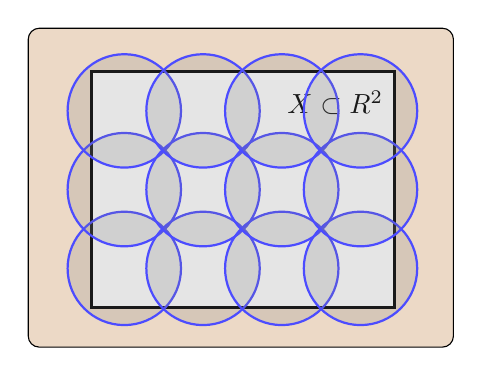
\begin{tikzpicture}%[overlay,remember picture,shift={(10.75,1.25)}]
\draw[fill=brown!30,rounded corners] (-1.3,-0.9) rectangle (4.1,3.15);


\draw[very thick,fill=white] (-0.5,-0.4) rectangle (3.35,2.6);
\node at (2.6,2.2) {$X \subset\mathbb{R}^2$};
\begin{scope}[shift={(-0.08,0.1)}]
%\clip (-0.4,-0.5) rectangle (3.45,2.5);
\foreach \x in {0,1,2,3}
  \foreach \y in {0,1,2}
    \draw[thick,blue!70,fill=gray,fill opacity=0.2] (\x,\y) circle (0.72);
\end{scope}
\end{tikzpicture}
\hspace{1cm}
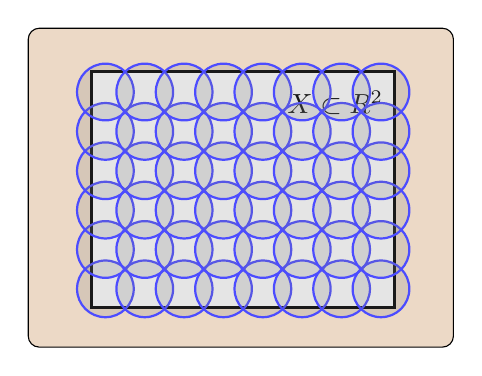
\begin{tikzpicture}%[overlay,remember picture,shift={(10.75,1.25)}]
\draw[fill=brown!30,rounded corners] (-1.3,-0.9) rectangle (4.1,3.15);


\draw[very thick,fill=white] (-0.5,-0.4) rectangle (3.35,2.6);
\node at (2.6,2.2) {$X \subset\mathbb{R}^2$};
\begin{scope}[shift={(-0.32,-0.16)}]
%\clip (-0.4,-0.5) rectangle (3.45,2.5);
\foreach \x in {0,0.5,1,1.5,2,2.5,3,3.5}
  \foreach \y in {0,0.5,1,1.5,2,2.5}
    \draw[thick,blue!70,fill=gray,fill opacity=0.2] (\x,\y) circle (0.36);
\end{scope}
\end{tikzpicture}

\end{center}



\item \textbf{Definition:} A metric space $(X,d)$ is \textbf{compact} if it is complete and totally bounded.


\item \textbf{Examples}
\begin{itemize} 
  \item The closed real interval $[0,1]\subset \bbR$ is compact
  \item A subset of Euclidean $\bbR^n$ is compact iff it is closed and bounded [Heine–Borel Theorem]
  \item But, the standard metric space of real numbers is not compact because it is not totally bounded.
\end{itemize}


\item \textbf{Theorem:} A closed subset $A$ of a compact space $X$ is itself a compact space.

\item \textbf{Example:}

\begin{itemize}
\item Any bounded and closed subset of $\bbR^n$ is compact
\item Let $A= \bbQ \cap [0,1]$ be the rationals in the unit interval. The set $A$ is a  bounded and closed subset of the rationals. However, the space $(A, d)$ is not compact because it is not complete. This example also highlights the distinction between closure and completeness. 
\end{itemize}


\item \textbf{Definition:}  Let $x_1,x_2,x_3\ldots \in X$ be a sequence and $n_1,n_2,n_3, \ldots\in \mathbb{N}$ be
a strictly increasing sequence
\[
n_1 < n_2 < \cdots < n_{k} < n_{k+1} 
\]
Then, $x_{n_k} = (x_{n_1},x_{n_2},\ldots)$ is a \textbf{subsequence} of $x_n$.


\item \textbf{Theorem:}  [Bolzano--Weierstrass]
A sequence in a compact metric space has a subsequence that converges.


\item \textbf{Example:} Compact metric space $X=[-2,2]\subset \mathbb{R}$ with absolute distance. Define squence
\[
 x_n = (-1)^n + \frac{1}{n}
 \]
\begin{itemize}
\item subsequence with even indices $x_2,x_4,x_6,\ldots$ converges to 1.
\item subsequence with odd indices converges to $-1$ 
\end{itemize}


\item \textbf{Proof:} Bolzano--Weierstrass% for closed real line. 
\begin{itemize}
\item Let $x_n$ be sequence in Compact set $X$%= [ a, b] \subset \bbR$.

\item A subset $A \subset X$ contains (countably) infinitely many terms in the sequence if
\[
 | \{ n \in \bbN \mid x_n \in A \} | = \infty 
\]
\item We first argue that for any  $k  \in \bbN$, there exists a subset $A_k \subseteq X$ such that 
\[
 | \{ n \in \bbN \mid x_n \in A_k \} | = \infty  \qquad \text{and} \qquad  \forall x, y \in A_k, \quad  d(x,y)  < 1/k 
% | \{ n \in \bbN \mid x_n \in [a',b']  \} | = \infty  \qquad \text{and} \qquad  |b'-a'| \le \eps
\]
This holds because the space is \emph{totally bounded} and thus for $\eps = 1/(2k)$, the set $X$ can be covered by a finite number of open $\eps$-balls. At least one of these balls must contain an infinite number of terms in the sequence, and so at least one choice of $A_k$ exists. 

\item If we define $n^k_1, n^k_2, n^k_3, \dots \in \bbN$  to the time indices in which $x_n \in A_k$, then the subsequence $x_{n^k_1}, x_{n^k_2}, x_{n^k_3}, \dots$ satisfies
\[
\forall i, j \in \bbN, \quad  d(x_{n_i^k},x_{n_j^k} )  < 1/k 
\]

\item But in order to show that subsequence Cauchy, we need to show that that that terms are (eventually) no more than $\eps$ apart for \emph{any} $\eps > 0$, not just the choice $1/k$ constructed above. 

\item The solution is to apply the argument above recursively to define a decreasing sequence of sets $X \supseteq A_1  \supseteq A_2 \supseteq \cdots \supseteq A_k$.  Then, we consider the subsequence defined by that $k$-th arrival in the $k$-th subset, 
\[
x_{n_1^1}, x_{n_2^2},  x_{n_3^3}, \dots
\]
Here it is easy to check that  the indices are strictly increasing, i.e., $n_1^1 <  n_2^2  < \cdots  < n_k^k  < n_{k+1}^{k+1}$, and so this is a valid subsequence. 

\item Then, for every $\eps > 0$, there exists $N_\eps = \lceil 1/\eps \rceil$ such that  %we see that
\[
i, j \ge N_\eps  \qquad \implies \quad d(x_{n_i^i}, x_{n_j^j})  < \eps 
\]
 and so the subsequence is Cauchy!
 
 \item Since the space is complete, every Cauchy sequence is convergent. 


\end{itemize}



\item \textbf{Theorem:}  Let $X$ be a metric space and $f \colon X\rightarrow \bbR$ be a continuous function from $X$ to $\mathbb{R}$. If $A$ is a compact subset of $X$, then there exists $x\in A$ such that $f(x)=\sup f(A)$ (i.e., $f$ achieves a maximum on $A$).
% \gpt{Suggested cut/paste hypothesis: require $A$ to be nonempty and compact.}

\item \textbf{Theorem:}  
Let $(X,d)$ be a compact metric space and $C(X)$ be the set of continuous functions mapping $X$ to $\mathbb{R}$.
This set of functions, with the metric 
 \[
 d_\infty (f,g) \coloneqq \sup_{x\in X} |f(x)-g(x)| = \max_{x\in X} |f(x)-g(x)|,
 \] defines a complete metric space.


\item \textbf{Note:}  Note: For $f,g\in C(X)$, $d_\infty$ metrizes uniform convergence because 
\[
\max_{x\in X} |f(x)-g(x)| < \epsilon  \quad \iff \quad  \forall x\in X, \;  |f(x) - g(x)| < \epsilon
 \]


\end{itemize}







\bibliographystyle{alpha}%{IEEEtran}
\bibliography{/Users/galenreeves/Dropbox/Library/long_names,/Users/galenreeves/Dropbox/Library/library} 
\end{document}
